\chapter{身体构型与共同祖先}\label{ch:g10:common-ancestry}

伸出你的手臂数一数：从肩到肘是一块骨，
从肘到腕是两块骨，腕部是一簇小骨，然后是五根手指。现在
看看蝙蝠翅膀、鲸的鳍肢、马的前腿、青蛙前肢的骨骼：
它们都是同样的一块骨、两块骨、一簇小骨和指（趾）节，
有的拉长，有的融合，有的缩短，却从不被重新排列。没有人
从零开始设计翅膀时会以手臂为起点。这种相似性
正是遗传的标志。本章要讨论的，是如何从骨骼、胚胎和分子中
读取这些标志，据此重建
生物之间的亲缘关系。

\section{脊椎动物的身体构型}

\begin{definition}[身体构型]\label{def:g10:common-ancestry:bodyplan}
一类生物的\emph{身体构型}\index{身体构型}，是指其各部分的
共同排列方式：对称轴以及主要器官的相对位置，
与体型、形状或生活方式无关。\emph{脊椎动物}\index{脊椎动物}
——鱼类、两栖动物、爬行动物、鸟类和哺乳动物——共享同一种构型：
身体沿竖直平面对称，前端为头，后端为尾；
内骨骼的中轴是一列椎骨，
保护背侧的神经索；
消化管位于腹侧，
口在前方，心脏位于其下方。
\end{definition}

\begin{omfigure}
\begin{tikzpicture}[font=\small, >=Stealth]
  % generic vertebrate side view
  \draw[thick, fill=omDef!6, rounded corners=14pt] (0,0) rectangle (9,3.2);
  \draw[thick, omThm] (0.6,2.5) -- (8.6,2.5);                      % nerve cord
  \foreach \x in {1.2,1.8,...,8.4} \draw[thick] (\x,2.15) -- (\x,2.35); % vertebrae
  \draw[thick] (1.0,2.25) -- (8.6,2.25);
  \draw[thick, omProp, fill=omProp!20] (0.5,1.4) .. controls (2,0.7) and (6,0.7) .. (8.6,1.2)
    .. controls (6,1.5) and (2,1.9) .. (0.5,1.4);                      % gut
  \draw[thick, omThm, fill=omThm!30] (2.3,0.75) circle (0.32);         % heart
  \node[anchor=west] at (9.4,2.5) {神经索（背侧）};
  \draw[->] (9.35,2.5) -- (8.65,2.5);
  \node[anchor=west] at (9.4,2.0) {脊柱};
  \draw[->] (9.35,2.0) -- (8.6,2.22);
  \node[anchor=west] at (9.4,1.2) {消化管（腹侧）};
  \draw[->] (9.35,1.2) -- (8.65,1.2);
  \node[anchor=north] at (2.3,-0.1) {心脏，位于消化管下方};
  \draw[->] (2.3,-0.05) -- (2.3,0.4);
  \node[anchor=east] at (-0.1,1.4) {口};
  \draw[->] (-0.05,1.4) -- (0.45,1.4);
  \node[anchor=south, font=\small\itshape] at (4.5,3.3) {背侧};
  \node[anchor=north, font=\small\itshape] at (6.5,-0.05) {腹侧};
  \draw[<->, gray] (0,3.7) -- (9,3.7) node[midway, above, font=\scriptsize] {前后轴};
\end{tikzpicture}

{\small \omterm{def:g10:common-ancestry:bodyplan}{脊椎动物}\omterm{def:g10:common-ancestry:bodyplan}{身体构型}的侧视图。无论是哪个\omterm{def:g10:biodiversity-scales:species}{物种}，
神经索都沿背部位于脊柱上方，消化管沿腹部走向，
心脏位于其下方靠近前端处。昆虫和蚯蚓的神经索
位于腹侧，属于
不同的构型。}
\end{omfigure}

\begin{example}[同一构型，不同动物]\label{ex:g10:common-ancestry:sameplan}
将鳟鱼、青蛙、蜥蜴、鸽子和小鼠并排解剖，
每一种都显示出同样的构型：脊髓位于背部，由椎骨保护；
消化管位于其下方，肝脏紧邻胃；心脏位于前方、消化管下方；
成对的四肢（或鳍）连接在骨质带上。
它们的差异——鳃或肺、鳍或腿、鳞片、羽毛或皮毛——
都是在同一种排列基础上的变化。
\end{example}

\section{同源器官}

\begin{definition}[同源]\label{def:g10:common-ancestry:homology}
两个\omterm{def:g10:biodiversity-scales:species}{物种}的两个器官，若\emph{同源}\index{同源}，
结构相同、在\omterm{def:g10:common-ancestry:bodyplan}{身体构型}中的位置相同——由相同部件以相同关系构成——
无论其现在的功能如何，
四足动物的前肢是典型例子：
一块骨（肱骨）、两块骨（桡骨和尺骨）、一簇腕骨，
然后是指（趾）节。执行相同功能而结构不同的器官
——鸟的翅膀与蝇的翅膀——仅为
\emph{同功}，与亲缘关系无关。
\end{definition}

\begin{omfigure}
\begin{tikzpicture}[font=\small, line cap=round]
  % three stylised forelimbs: humerus (red), radius+ulna (blue), carpals (gray), digits (green)
  \tikzset{hum/.style={line width=6pt, omThm!70},
           ru/.style={line width=4pt, omDef!70},
           carp/.style={fill=gray!50, draw=gray!70},
           dig/.style={line width=3pt, omMeth!80}}
  % human arm
  \begin{scope}
    \draw[hum] (0,3.2) -- (0.2,1.9);
    \draw[ru] (0.1,1.85) -- (0.3,0.9); \draw[ru] (0.35,1.85) -- (0.5,0.9);
    \fill[carp] (0.15,0.7) rectangle (0.65,0.85);
    \foreach \dx in {-0.3,-0.12,0.05,0.22,0.4} \draw[dig] (0.4,0.7) -- ({0.4+\dx},-0.1);
    \node[anchor=north] at (0.4,-1.4) {人的手臂};
  \end{scope}
  % bat wing
  \begin{scope}[xshift=3.6cm]
    \draw[hum] (0,3.2) -- (0.4,2.3);
    \draw[ru] (0.4,2.3) -- (1.0,1.3);
    \fill[carp] (0.95,1.2) rectangle (1.25,1.35);
    \draw[dig] (1.1,1.2) -- (0.8,0.9);
    \foreach \a in {-0.6,-0.3,0.1,0.5} \draw[dig] (1.1,1.2) -- ({1.1+2.2*cos(-60+40*\a)},{1.2+2.2*sin(-60+40*\a)});
    \node[anchor=north] at (1.2,-1.4) {蝙蝠翅膀};
  \end{scope}
  % whale flipper
  \begin{scope}[xshift=8.0cm]
    \draw[hum] (0,3.2) -- (0.1,2.5);
    \draw[ru] (0.0,2.45) -- (0.05,1.9); \draw[ru] (0.3,2.45) -- (0.35,1.9);
    \fill[carp] (-0.05,1.6) rectangle (0.5,1.85);
    \foreach \dx in {-0.2,0.0,0.2,0.45} \draw[dig] ({0.22+0.5*\dx},1.6) -- ({0.22+\dx},0.2);
    \draw[gray!60, rounded corners=8pt] (-0.5,3.4) -- (-0.6,0.0) -- (0.9,-0.1) -- (0.9,3.4);
    \node[anchor=north] at (0.2,-1.4) {鲸的鳍肢};
  \end{scope}
  % legend
  \begin{scope}[xshift=10.4cm, yshift=2.2cm]
    \draw[hum] (0,1.0) -- (0.6,1.0); \node[anchor=west] at (0.7,1.0) {肱骨};
    \draw[ru] (0,0.5) -- (0.6,0.5); \node[anchor=west] at (0.7,0.5) {桡骨、尺骨};
    \fill[carp] (0.05,-0.08) rectangle (0.55,0.08); \node[anchor=west] at (0.7,0) {腕骨};
    \draw[dig] (0,-0.5) -- (0.6,-0.5); \node[anchor=west] at (0.7,-0.5) {指（趾）节};
  \end{scope}
\end{tikzpicture}

{\small 三条\omterm{def:g10:common-ancestry:homology}{同源}前肢示意：骨骼相同，
排列次序相同，有的拉长成翅膀，有的压扁成鳍状肢。
功能不同，结构和位置却相同。}
\end{omfigure}

\begin{omfigure}
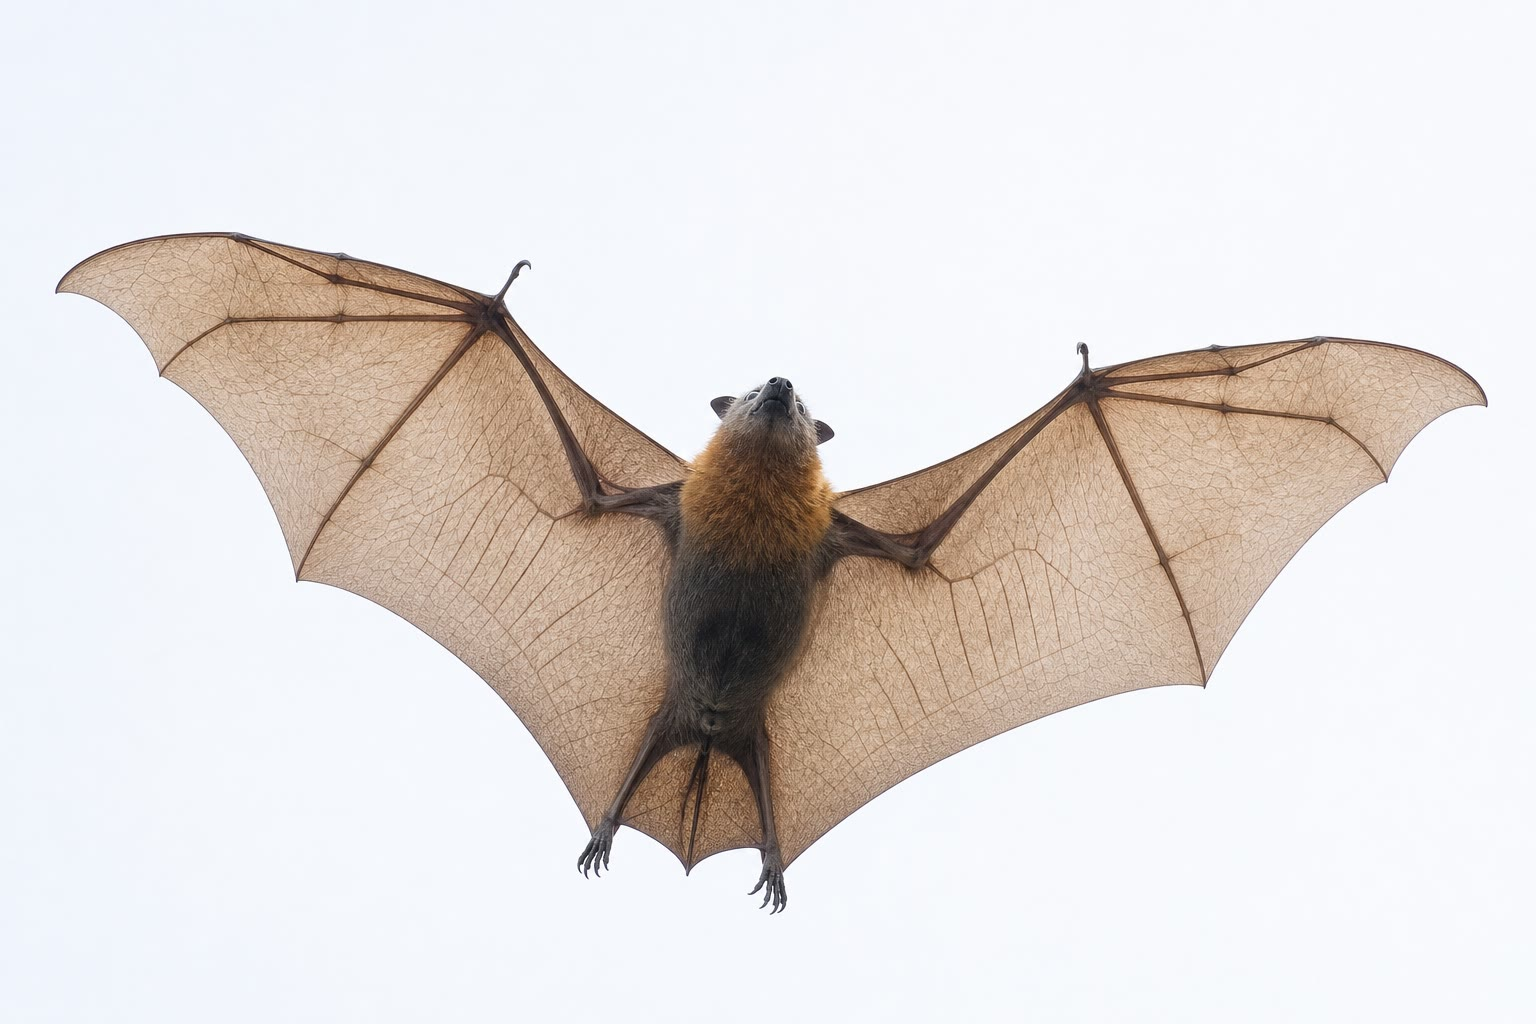
\includegraphics[width=0.6\linewidth]{images/book2/ai/g10-ancestry-bat-wing.jpg}

{\small 飞行中的蝙蝠：翼膜绷在
极度拉长的指骨之上。哺乳动物的手，
变成了翅膀。}
\end{omfigure}

\begin{proposition}[同源性揭示亲缘关系]\label{prop:g10:common-ancestry:kinship}
共有的\omterm{def:g10:common-ancestry:homology}{同源}结构，由拥有它们的共同祖先遗传而来；
两个\omterm{def:g10:biodiversity-scales:species}{物种}共有的此类结构越多，二者的亲缘关系就越近。
四足动物的肢见于每一种陆生\omterm{def:g10:common-ancestry:bodyplan}{脊椎动物}，
因为它们都源自一个具有此肢的祖先谱系；
蝙蝠的翅膀是经过改造的手臂，因为蝙蝠源自具有手臂的哺乳动物，
而非源自鸟类。
\end{proposition}
\begin{proof}[证据]
三条相互独立的证据指向同一结论。\emph{化石}：按年代顺序排列的
岩层中含有兼具多种性状的中间类型——
375 百万年前的鱼类，有类似肢的鳍和颈，随后
出现有鱼类样尾巴的四足动物；\emph{始祖鸟}，
150 百万年前，有羽毛和翅膀，但也有牙齿、带爪的
指和长而有骨节的尾巴。\emph{胚胎}：所有\omterm{def:g10:common-ancestry:bodyplan}{脊椎动物}的胚胎
都经历一个具有鳃裂、尾巴和脊索的阶段——
这些结构在成年鱼类中保留，在其他动物中则被改造或消失。
\emph{分子}：如\cref{ch:g10:universal-dna}所示，所有生物共有
\omterm{def:g10:universal-dna:information}{DNA} 和相同的\omterm{def:g10:universal-dna:gene}{基因}，同一\omterm{def:g10:universal-dna:gene}{基因}不同版本之间的差异，
其排列次序与解剖学结果完全一致。
\end{proof}

\begin{omfigure}
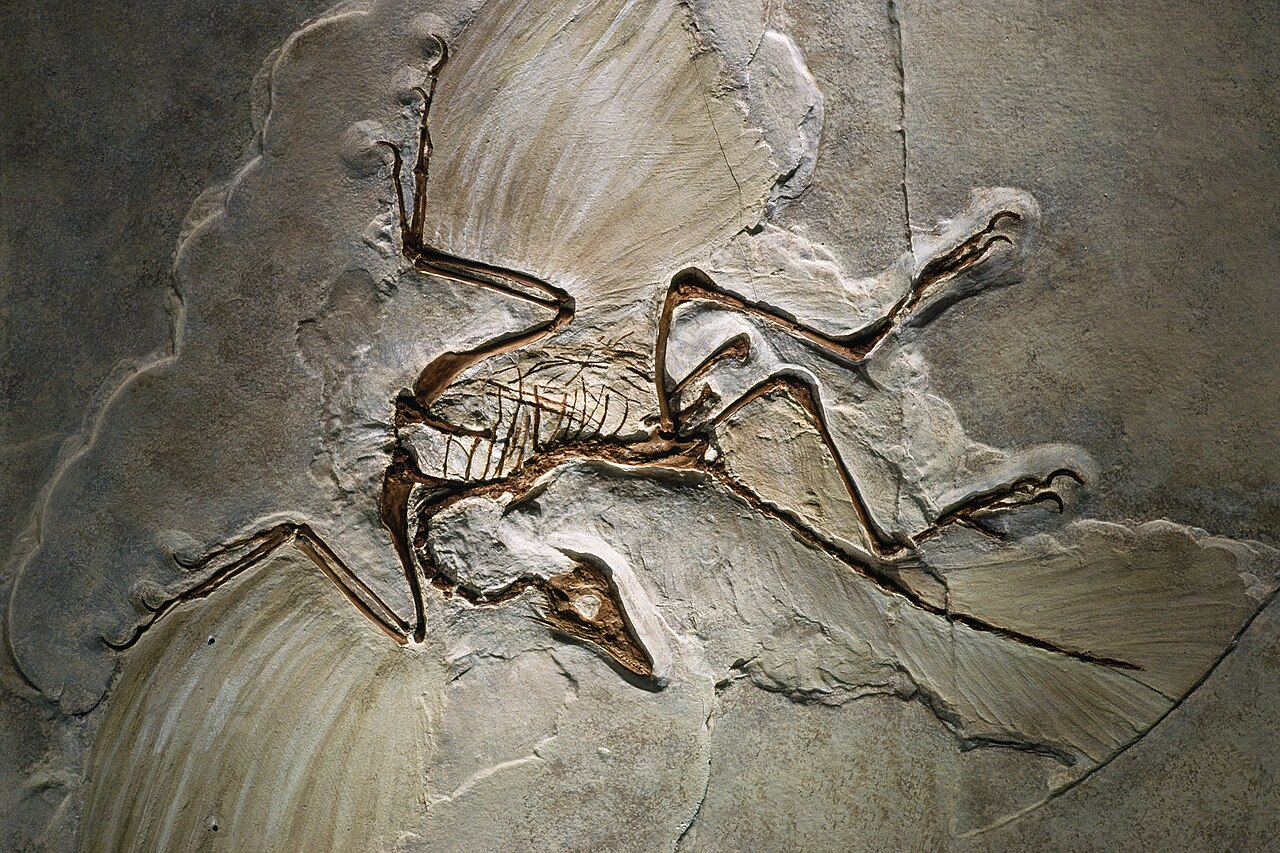
\includegraphics[width=0.5\linewidth]{images/book1/archaeopteryx.jpg}

{\small \emph{始祖鸟}，150 百万年前：羽翼和叉骨与鸟类相似，
同时有牙齿、带爪的指，以及如小型恐龙一般长而有骨节的
尾巴。兼具两类群特征的化石，
正是共同祖先理论所预测的。照片：James L.~Amos，CC0。}
\end{omfigure}

\section{嵌套类群}

\begin{method}[依共有性状分组]\label{met:g10:common-ancestry:grouping}
亲缘类群依共有的\emph{衍生}性状划分——
即在某一祖先中一次性出现、并被其
全部后代遗传的性状。
\begin{enumerate}
  \item 列出\omterm{def:g10:biodiversity-scales:species}{物种}及一组性状（脊柱；
        四肢；带壳卵或其等价物，即羊膜卵；
        羽毛；毛发与乳汁；等等）。
  \item 对每一性状，记录哪些\omterm{def:g10:biodiversity-scales:species}{物种}具有该性状。
  \item 由某一子集共有的性状定义一个类群：所有具有
        四肢的\omterm{def:g10:biodiversity-scales:species}{物种}为四足动物；其中，所有具有
        羊膜卵的为羊膜动物；在其中，所有具有毛发的
        为哺乳动物。
  \item 将各类群画成嵌套的方框，或画成树状图，其中每个
        节点是该性状首次出现的共同祖先。
        一个类群必须包含该祖先的\emph{全部}后代：
        日常所说的“鱼类”或“爬行动物”
        并不是这样的类群。
\end{enumerate}
\end{method}

\begin{omfigure}
\begin{tikzpicture}[font=\small]
  \node[draw, rounded corners, thick, fill=omDef!6, minimum width=12.2cm, minimum height=4.6cm] (v) at (0,0) {};
  \node[anchor=north west] at (v.north west) {\ \textbf{脊椎动物}：脊柱};
  \node[anchor=south west] at (v.south west) {\ 鳟鱼};
  \node[draw, rounded corners, thick, fill=omMeth!8, minimum width=9.6cm, minimum height=3.5cm] (t) at (0.9,-0.25) {};
  \node[anchor=north west] at (t.north west) {\ \textbf{四足动物}：四肢};
  \node[anchor=south west] at (t.south west) {\ 青蛙};
  \node[draw, rounded corners, thick, fill=omProp!10, minimum width=7.0cm, minimum height=2.4cm] (a) at (1.8,-0.5) {};
  \node[anchor=north west] at (a.north west) {\ \textbf{羊膜动物}：羊膜卵};
  \node[anchor=south west] at (a.south west) {\ 蜥蜴\quad 鸽子};
  \node[draw, rounded corners, thick, fill=omThm!10, minimum width=3.7cm, minimum height=1.3cm] (m) at (3.2,-0.75) {};
  \node[anchor=north west] at (m.north west) {\ \textbf{哺乳动物}：毛发、乳汁};
  \node[anchor=south west] at (m.south west) {\ 小鼠\quad 人};
\end{tikzpicture}

{\small 五种\omterm{def:g10:common-ancestry:bodyplan}{脊椎动物}的嵌套亲缘类群。每个方框由
一个仅出现一次的性状定义，该性状出现在方框内
所有生物的共同祖先中。鸽子与蜥蜴同属“羊膜动物”，蜥蜴
与鸽子的亲缘关系比与青蛙的更近。}
\end{omfigure}

\begin{example}[读懂方框]\label{ex:g10:common-ancestry:reading}
在鳟鱼、青蛙、蜥蜴和鸽子中，哪一种与小鼠的亲缘关系最近？
包含小鼠及另一\omterm{def:g10:biodiversity-scales:species}{物种}的最小方框是
“羊膜动物”，其中有蜥蜴和鸽子：二者与小鼠的距离相等，
二者都比青蛙更接近小鼠，而青蛙又
比鳟鱼更接近。蜥蜴与鸽子的关系比与青蛙的更近，
这让大多数人感到意外；
带壳卵是青蛙所没有的性状，它说明了这一点。
\end{example}

\section{分子中的亲缘关系}

\begin{proposition}[分子亲缘关系]\label{prop:g10:common-ancestry:molecular}
既然所有生物都源自共同祖先，则两个\omterm{def:g10:biodiversity-scales:species}{物种}中都存在的某一\omterm{def:g10:universal-dna:gene}{基因}，
是祖先\omterm{def:g10:universal-dna:gene}{基因}的改造副本；两份副本之间的差异数，
随\omterm{def:g10:biodiversity-scales:species}{物种}分化以来的时间增长而增加。
比较不同\omterm{def:g10:biodiversity-scales:species}{物种}中某一\omterm{def:g10:universal-dna:gene}{基因}，或其所编码
的\omterm{def:g10:chemistry-of-life:families}{蛋白质}的序列，即可度量亲缘关系；
由此得到的分组与依解剖学划分的结果一致。
\end{proposition}
\admitted

\begin{example}[细胞色素 c]\label{ex:g10:common-ancestry:cytochrome}
\omterm{def:g10:cells-common-unit:cell}{细胞}色素 c 是一种约含 104 个\omterm{def:g10:chemistry-of-life:families}{氨基酸}的\omterm{def:g10:chemistry-of-life:families}{蛋白质}，
每种真核生物都用它参与呼吸作用。与人类序列相比，
黑猩猩的序列在 0 个位置上不同，小鼠的在 9 个位置，鸡的
在 13 个位置，青蛙的在 18 个位置，金枪鱼的在 21 个位置，酵母的在 45 个位置。
按差异数排序，各\omterm{def:g10:biodiversity-scales:species}{物种}恰好落入前图的各个方框：
哺乳动物，其次是羊膜动物，再次是四足动物，然后是\omterm{def:g10:common-ancestry:bodyplan}{脊椎动物}，
最后是真核生物。
\end{example}

\begin{remark}[统一性与亲缘关系]\label{rem:g10:common-ancestry:unity}
组成的统一性（\cref{ch:g10:chemistry-of-life}）、\omterm{def:g10:cells-common-unit:cell}{细胞}的统一性
（\cref{ch:g10:cells-common-unit}）、遗传分子的统一性
（\cref{ch:g10:universal-dna}）以及现在的\omterm{def:g10:common-ancestry:bodyplan}{身体构型}和\omterm{def:g10:universal-dna:gene}{基因}序列的统一性，
是同一事实的四种表现：生物彼此相似，是因为它们有亲缘关系；
它们有亲缘关系，是因为它们源自共同祖先。
\cref{ch:g10:biodiversity-scales}中的多样性，
是携带变异的世代传承在
化石记录所度量的时间里的结果。变异如何产生和扩散，
是最后一年课程的内容。
\end{remark}

\section{练习}

\begin{exercise}[$\star$]\label{exo:g10:common-ancestry:1}
列出\omterm{def:g10:common-ancestry:bodyplan}{脊椎动物}\omterm{def:g10:common-ancestry:bodyplan}{身体构型}的四个特征。
\end{exercise}

\begin{exercise}[$\star$]\label{exo:g10:common-ancestry:2}
定义\omterm{def:g10:common-ancestry:homology}{同源}器官，并给出标准例子。
\end{exercise}

\begin{exercise}[$\star$]\label{exo:g10:common-ancestry:3}
鸟的翅膀与蝴蝶的翅膀是\omterm{def:g10:common-ancestry:homology}{同源}的还是同功的？
请说明理由。
\end{exercise}

\begin{exercise}[$\star$]\label{exo:g10:common-ancestry:4}
利用嵌套方框图，判断在鳟鱼与蜥蜴中，
哪一种与青蛙的亲缘关系更近。
\end{exercise}

\begin{exercise}[$\star$]\label{exo:g10:common-ancestry:5}
哪三类证据支持共享\omterm{def:g10:common-ancestry:homology}{同源}特征
源自共同祖先这一观点？
\end{exercise}

\begin{exercise}[$\star\star$]\label{exo:g10:common-ancestry:6}
鲸有一个具四足动物骨骼模式的鳍肢，用肺呼吸，
哺乳幼体，并有与任何腿都不相连的微小髋骨。
它属于图中的哪个方框？髋骨说明了什么？
\end{exercise}

\begin{exercise}[$\star\star$]\label{exo:g10:common-ancestry:7}
把鳄鱼（四肢、羊膜卵、鳞片、无毛）和
蝾螈（四肢、在水中产无壳卵）
一并加入嵌套方框中。
\end{exercise}

\begin{exercise}[$\star\star$]\label{exo:g10:common-ancestry:8}
解释为什么“鱼类”（鳟鱼、鲨鱼、肺鱼……）按
\cref{met:g10:common-ancestry:grouping}的含义不是一个亲缘类群，
已知肺鱼与青蛙的亲缘关系比与鳟鱼更近。
\end{exercise}

\begin{exercise}[$\star\star$]\label{exo:g10:common-ancestry:9}
利用\omterm{def:g10:cells-common-unit:cell}{细胞}色素 c 的数据，将人的亲属按亲缘关系
由近到远排序，并与解剖学方框的划分进行核对。
\end{exercise}

\begin{exercise}[$\star\star$]\label{exo:g10:common-ancestry:10}
四周龄的人类胚胎在颈部有鳃囊，并有一条尾巴，
两者之后都会消失。这一观察对
本章的论证有何贡献？
\end{exercise}

\begin{exercise}[$\star\star$]\label{exo:g10:common-ancestry:11}
\emph{Archaeopteryx} 有羽毛和一条长的带骨尾巴。解释为什么
在共同祖先假设下，人们预期会找到兼具多种特征的化石，
而没有这一假设，这样的化石会令人困惑。
\end{exercise}

\begin{exercise}[$\star\star\star$]\label{exo:g10:common-ancestry:12}
章鱼与人类的眼睛都是带有透镜和
视网膜的照相机式结构，却由不同的组织发育而来，章鱼的
视网膜连接方式正好相反。二者是\omterm{def:g10:common-ancestry:homology}{同源}还是同功？
各自的答案对它们的共同祖先意味着什么？
\end{exercise}

\begin{exercise}[$\star\star\star$]\label{exo:g10:common-ancestry:13}
\omterm{def:g10:cells-common-unit:cell}{细胞}色素 c 在人与小鼠之间有 9 个位置不同，在人与鸡之间有
13 个位置不同，小鼠与鸡之间也有 13 个位置不同。
解释为什么后两个数字预期应相等（或接近相等），
若差异随时间稳定积累。
\end{exercise}

\begin{exercise}[$\star\star\star$]\label{exo:g10:common-ancestry:14}
蛇没有四肢，却被归入四足动物。
依据是什么？那么“四足动物”一词又指什么？
\end{exercise}

\begin{exercise}[$\star\star\star$]\label{exo:g10:common-ancestry:15}
一位朋友认为，相似的动物只是生活方式相似，
所以外形才相似。利用前肢、胚胎和
分子，解释这一说法无法说明什么。
\end{exercise}

\section{问题：同一棵树，两类证据}

\begin{problem}[{周末问题——五种脊椎动物、它们的骨骼与其中一种蛋白质：
由解剖学建立亲缘关系，由分子重建亲缘关系，
并比较两者}]
\label{pb:g10:common-ancestry:1}
班级研究五个\omterm{def:g10:biodiversity-scales:species}{物种}：鳟鱼、青蛙、蜥蜴、鸽子和
小鼠。特征表（1 = 存在，0 = 不存在）：

\begin{center}
\begin{tabular}{lccccc}
 & 鳟鱼 & 青蛙 & 蜥蜴 & 鸽子 & 小鼠 \\ \hline
脊柱 & 1 & 1 & 1 & 1 & 1 \\
四肢 & 0 & 1 & 1 & 1 & 1 \\
羊膜卵 & 0 & 0 & 1 & 1 & 1 \\
羽毛 & 0 & 0 & 0 & 1 & 0 \\
毛发和乳汁 & 0 & 0 & 0 & 0 & 1 \\
\end{tabular}
\end{center}

\omterm{def:g10:cells-common-unit:cell}{细胞}色素 c 的差异数（取整）：

\begin{center}
\begin{tabular}{lcccc}
 & 青蛙 & 蜥蜴 & 鸽子 & 小鼠 \\ \hline
鳟鱼 & 19 & 20 & 21 & 21 \\
青蛙 & & 16 & 17 & 18 \\
蜥蜴 & & & 12 & 14 \\
鸽子 & & & & 13 \\
\end{tabular}
\end{center}

\medskip
\noindent\textbf{第一部分——骨骼。}
\begin{enumerate}
  \item 哪一种特征为五种动物所共有？它
        定义了哪一个类群？
  \item 哪些特征分别定义了一个由四种动物组成的类群、一个由三种动物组成的类群？
        写出这些类群的名称。
  \item 羽毛和毛发各只见于一个\omterm{def:g10:biodiversity-scales:species}{物种}。这样的特征能否
        在这五种动物中定义一个亲缘类群？它
        有什么用处？
  \item 画出五个\omterm{def:g10:biodiversity-scales:species}{物种}的嵌套方框图，或
        画出与之对应的系统树。
  \item 青蛙的前肢具有肱骨、桡尺骨、腕和指的结构；
        鳟鱼的胸鳍则由一小段基部向外辐射排列的骨条构成。
        哪一个与你的手臂\omterm{def:g10:common-ancestry:homology}{同源}？
        这对应表中的哪一个特征？
\end{enumerate}

\medskip
\noindent\textbf{第二部分——分子。}
\begin{enumerate}[resume]
  \item 根据第二张表，哪两个\omterm{def:g10:biodiversity-scales:species}{物种}是最近的一对？
        哪一个\omterm{def:g10:biodiversity-scales:species}{物种}与所有其他\omterm{def:g10:biodiversity-scales:species}{物种}的距离最远？
  \item 将小鼠的各亲缘\omterm{def:g10:biodiversity-scales:species}{物种}按由近到远排序，
        仅利用分子信息。
  \item 对青蛙做同样的排序。这一排序与
        第一部分中的方框是否一致？
  \item 蜥蜴与鸽子之间的距离（12）小于蜥蜴与
        小鼠之间的距离（14）。这说明羊膜动物内部的
        分支顺序如何？表中的特征
        对此有无说明？
  \item 解释为什么鳟鱼与其他四种动物的距离
        都大致相等（19--21）。
\end{enumerate}

\medskip
\noindent\textbf{第三部分——两类证据的比较。}
\begin{enumerate}[resume]
  \item 列出两类证据一致支持的分组。
  \item 为什么解剖学排序与分子排序一致，
        就是有力的证据，而单独任何一类
        都可能受到质疑？
  \item 假设增加第六个\omterm{def:g10:biodiversity-scales:species}{物种}——蝙蝠：前肢具有
        四足动物的结构，有羊膜卵，有毛发和乳汁，\omterm{def:g10:cells-common-unit:cell}{细胞}色素 c
        与小鼠相差 8 个位点，与鸽子相差
        13 个位点。它应归入哪里？为什么它的翅膀
        不使它与鸽子归为一组？
  \item 黑猩猩的\omterm{def:g10:cells-common-unit:cell}{细胞}色素 c 与人的完全相同，
        但两个\omterm{def:g10:biodiversity-scales:species}{物种}在外观上明显不同。这说明
        \omterm{def:g10:cells-common-unit:cell}{细胞}色素 c 的比较能提供哪些\omterm{def:g10:universal-dna:gene}{基因}方面的信息，
        又不能提供哪些？
  \item 酵母的\omterm{def:g10:cells-common-unit:cell}{细胞}色素 c 与这五种动物的差异都在约 45
        个位点左右。哪一个比“\omterm{def:g10:common-ancestry:bodyplan}{脊椎动物}”更大的类群，
        是酵母与这五种动物共有的？
\end{enumerate}

\medskip
\noindent\textbf{第四部分——时间与系统树。}
化石记录表明，小鼠与鸽子两个谱系的分化
发生于约 3.2 亿年前。
\begin{enumerate}[resume]
  \item 若两个谱系的差异都稳定积累，沿一个谱系
        每 1 亿年会出现多少个差异？
        （利用小鼠与鸽子之间的距离，并注意两个
        谱系都在变化。）
  \item 利用该速率，估算青蛙谱系与羊膜动物
        的分化时间，依据
        青蛙与小鼠、青蛙与鸽子之间的距离。
  \item 同样估算鳟鱼谱系的分化时间。
  \item 化石表明，最早的四足动物出现于约 3.7 亿年
        前，最早的有颌\omterm{def:g10:common-ancestry:bodyplan}{脊椎动物}则远在 4.2 亿年以前。将其与
        你的估算结果相比较，并评论两者的吻合程度。
  \item 用一句话概括两类证据合在一起，
        确立了这五个\omterm{def:g10:biodiversity-scales:species}{物种}之间的何种关系，
        以及分子证据补充了骨骼所无法提供的哪些信息。
\end{enumerate}
\end{problem}
